\section{Verifica della convergenza dell'ottimizzazione}
\label{app:convergenza_turbojet}

Data la natura stocastica dell'algoritmo genetico, la robustezza delle
soluzioni è stata verificata mediante 150 esecuzioni indipendenti con
differenti popolazioni iniziali. L'andamento del minimo cumulativo della
funzione obiettivo è riportato in Figura~\ref{app:fig:cumulative_min_turbojet}
per il turbogetto e in Figura~\ref{app:fig:cumulative_min_ramjet}
per il ramjet.

\begin{figure}[H]
    \centering
    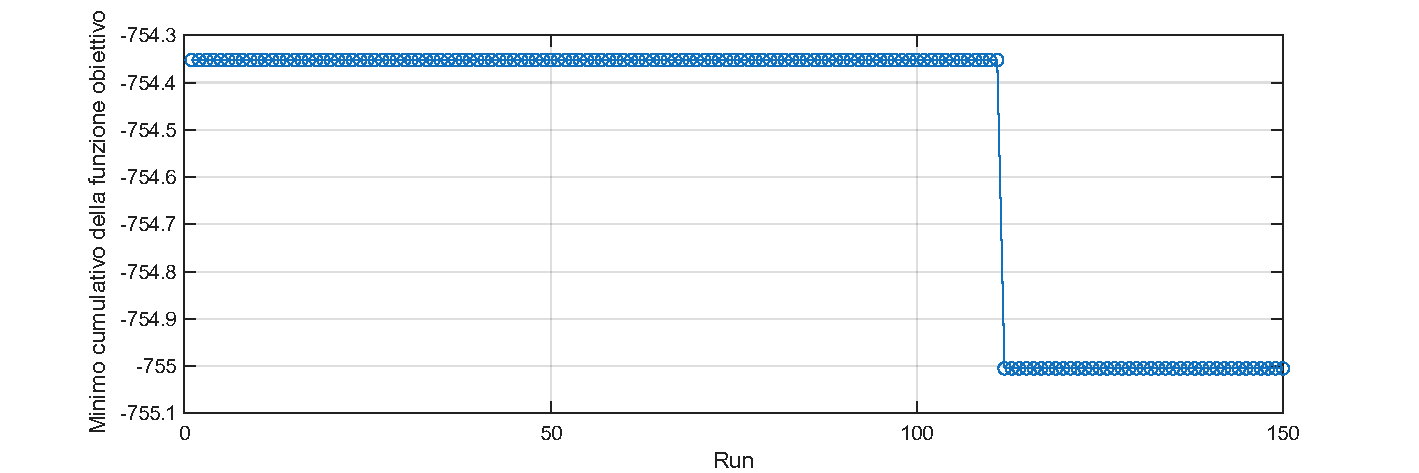
\includegraphics[width=1.1\linewidth]
    {Graphics/turbogetto/prestazioni/minimo_comulativo2.pdf}
    \caption{Andamento del minimo cumulativo della funzione obiettivo
    nelle 150 esecuzioni indipendenti dell'ottimizzazione del turbogetto.}
    \label{app:fig:cumulative_min_turbojet}
\end{figure}

\begin{figure}[H]
    \centering
    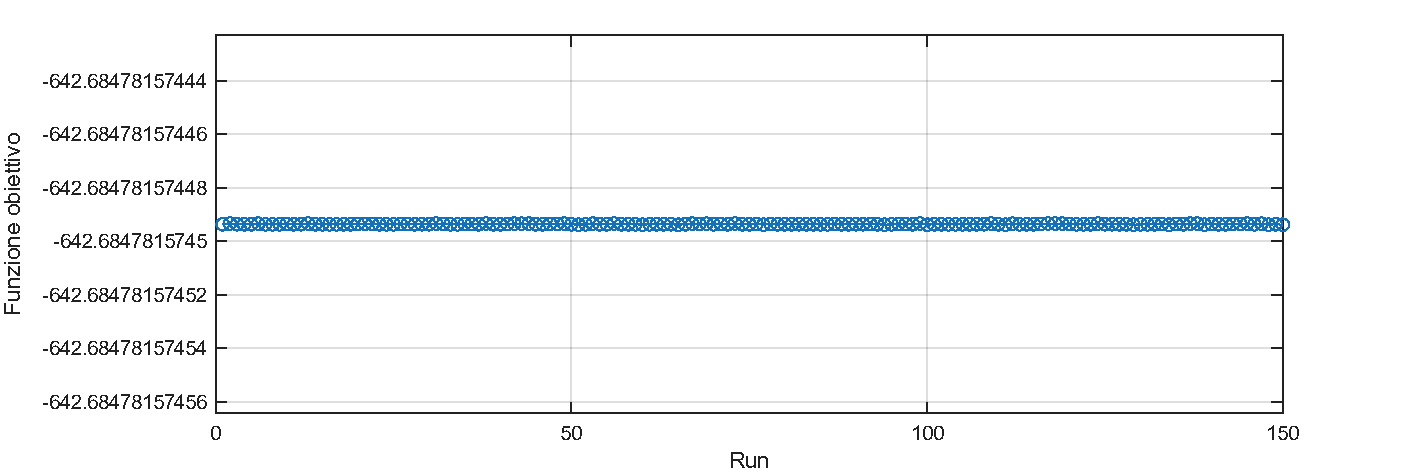
\includegraphics[width=1.1\linewidth]
    {Graphics/turbogetto/prestazioni/minimo_comulativo_ramjet}
    \caption{Andamento del minimo cumulativo della funzione obiettivo
    nelle 150 esecuzioni indipendenti dell'ottimizzazione del ramjet.}
    \label{app:fig:cumulative_min_ramjet}
\end{figure}

In entrambi i casi, la progressiva stabilizzazione del minimo cumulativo
mostra che l'aumento del numero di esecuzioni non determina ulteriori
riduzioni significative della funzione obiettivo. Tale comportamento
fornisce un'indicazione della limitata dipendenza delle soluzioni finali
dalle popolazioni iniziali.


%------------------------------------------
\section{Calcolo condizioni di volo turbogetto}
\label{app:appendiceA.1}
Le grandezze termodinamiche alla quota di volo $h=12000$ m possono essere calcolate utilizzando il modello dell'Atmosfera Standard Internazionale (ISA) dal quale si ricavano le seguenti grandezze statiche \cite{USStandardAtmosphere1976}.

\begin{align*}
    P_s = 19330 \, \text{Pa}\\
    T_s = 216.7 \,\text{K}
\end{align*}

Considerando un numero di Mach pari a $M =0.85$ imposto dalla missione, la velocità di volo risulta:

\begin{gather*}
    a = \sqrt{\gamma R T_s} = 295.1 \,\text{m/s}\\
    v_{\text{volo,tj}} = aM = 250.8 \,\text{m/s}
\end{gather*}

Calcolo delle grandezze totali
\begin{align*}
    T_{0}  &= T_s \left( 1 + \frac{\gamma-1}{2}M^2\right) = 248.0K \\
    P_{0}   &= P_s\left( 1 + \frac{\gamma-1}{2}M^2\right)^{\frac{\gamma}{\gamma-1}} = 30920Pa 
\end{align*}

\section{Calcolo delle condizioni di volo del ramjet}
Le grandezze termodinamiche alla quota di volo $h = 25000$ m vengono calcolate mediante il modello ISA:

\begin{gather*}
    P_s = 2549 \, \text{Pa}\\
    T_s = 221.7 \,\text{K}
\end{gather*}

Imponendo il numero di Mach di missione pari a $M = 3.5$ la velocità di volo risulta:

\begin{gather}
    a = \sqrt{\gamma R T_s} = 298.5 \,\text{m/s} \notag\\
    v_{\text{volo,rj}} = aM = 1045 \,\text{m/s}
    \label{eq:AppAVelocitàVoloRamjet}
\end{gather}

Le grandezze totali risultano:

\begin{align*}
    T_{0} &= T_s \left( 1 + \frac{\gamma-1}{2}M^2\right)
           = 765 \,\text{K} \\
    P_{0} &= P_s \left( 1 + \frac{\gamma-1}{2}M^2\right)^{\frac{\gamma}{\gamma-1}}
           = 194 \,\text{KPa}
\end{align*}

\section{Vincoli di volo ramjet}

La missione prevede una spinta totale di 65 kN. Il ramjet deve consumare al massimo $48000$ kg di carburante nella configurazione a due motori per coprire un range di $5000$ km alla velocità di volo calcolata \eqref{eq:AppAVelocitàVoloRamjet}. Pertanto un singolo motore deve consumare al massimo $m_{\text{c,disp}}$ = $24000$ kg di carburante.
Il tempo di missione può essere calcolato come

\begin{equation*}
    t_{\text{missione}} =
    \frac{\text{Range}}{v_{\text{volo,rj}}}
    = 4785 \,\text{s}
\end{equation*}

È quindi possibile calcolare la portata massima di carburante per completare la missione:

\begin{equation*}
    \dot{m}_{\text{c,max}} =
    \frac{m_{\text{c,disp}}}{t_{\text{missione}}}
    = 5.016 \,\text{kg/s}
\end{equation*}

Nota la spinta richiesta per il singolo motore, è possibile calcolare il TSFC massimo. 

\begin{equation*}
    TSFC_\text{max} =
    \frac{\dot{m}_{\text{c,max}} \cdot 3600}{F}
    = 0.2778 \,\text{kg/(Nh)}
\end{equation*}

\section{Spillamento d'aria per il raffreddamento della turbina}
\label{app:sezione:spillamentoArea}

Il raffreddamento della turbina è necessario per consentire il funzionamento ad alte temperature del motore. La portata d'aria richiesta può essere stimata a partire dalla temperatura SOT (Stator Outlet Temperature), calcolata in condizioni di blocco sonico del NGV (Nozzle Guide Vane) mediante la relazione \cite{slidesRobertoAndriani}:
\begin{equation}
    SOT = \frac{2}{\gamma_g+1}T_{04}
    \label{appA:eq:SOT}
\end{equation}

I dati di \cite{slidesRobertoAndriani} e la valutazione della $SOT$ tramite la Eq. \ref{appA:eq:SOT} permettono di determinare la frazione di aria spillata in funzione della temperatura di uscita dalla camera di combustione $T_{04}$, come mostrato in Figura \ref{appA:fig:frazioneDiAriaSpillata}.

\begin{figure} [H]
    \centering
    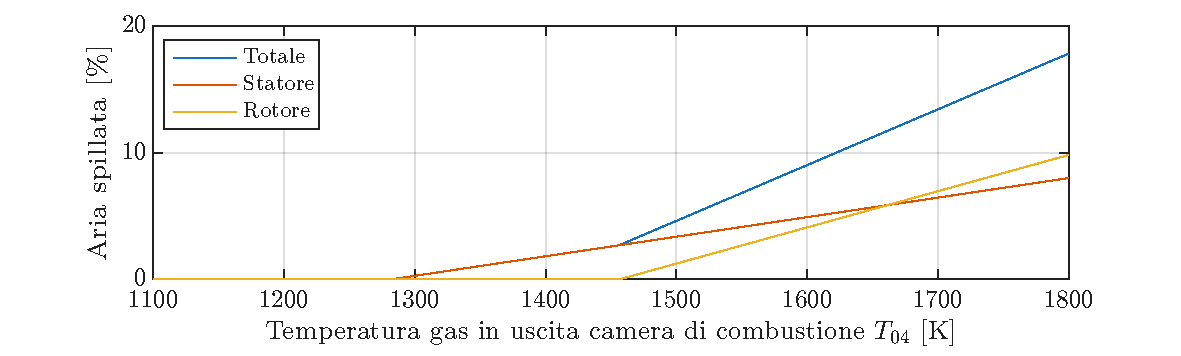
\includegraphics[width=0.9\linewidth]{Graphics/turbogetto/turbina/coolPercentagevsT04.pdf}
    \caption{Frazione di aria spillata dal compressore (\%) in funzione della temperatura $T_{04}$ [K].}
    \label{appA:fig:frazioneDiAriaSpillata}
\end{figure}

Posto il limite di $SOT \in [1100,1650] \text{ K}$, le funzioni analitiche per statore, rotore e totale che descrivono l'aria spillata dal compressore presentano la seguente formulazione in funzione della variabile di calcolo $SOT$:

\begin{equation*}
x_{\text{spillata, statore}}(\text{SOT}) = \begin{cases} 
0 & \text{se } \text{SOT} < 1100 \text{ K} \\ 
\frac{0.09}{550}(\text{SOT} - 1100) & \text{se } 1100 \le \text{SOT} \le 1650 \text{ K} 
\end{cases}
\end{equation*}

\begin{equation*}
x_{\text{spillata, rotore}}(\text{SOT}) = \begin{cases} 
0 & \text{se } \text{SOT} < 1250 \text{ K} \\ 
\frac{0.05}{350}(\text{SOT} - 1250) & \text{se } 1250 \le \text{SOT} \le 1650 \text{ K} \end{cases}
\end{equation*}

aria spillata totale dal compressore:
\begin{equation*}
x_{\text{spillata}}(\text{SOT}) = \begin{cases} 
0 & \text{se } \text{SOT} < 1100 \text{ K} \\ 
\frac{0.09}{550}(\text{SOT} - 1100) & \text{se } 1100 \le \text{SOT} < 1250 \text{ K} \\ 
\frac{0.09}{550}(\text{SOT} - 1100) + \frac{0.05}{350}(\text{SOT} - 1250) & \text{se } 1250 \le \text{SOT} \le 1650 \text{ K} \\ 
\end{cases}
\end{equation*}